\chapter{Designing the Data Capture System}
To obtain data for the Extended Kalman Filter, a data-capture system needed to be designed. Since the data sources have been identified as multiple video sources and a 9-DOF IMU.

\section{Camera Mount Design}


\begin{figure}
  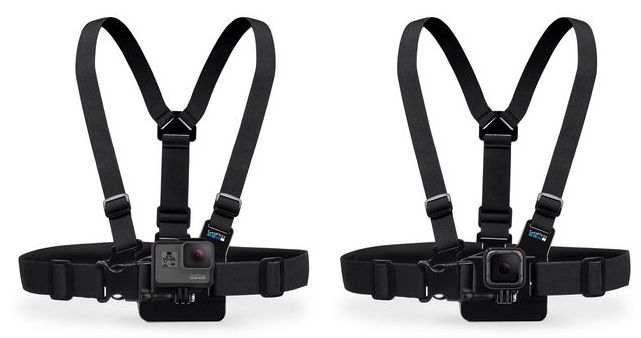
\includegraphics{figures/chesty.png}
  \caption{GoPro Chesty camera mount from \cite{chestygpwebsite}}
  \label{fig:chesty}
\end{figure}


\section{Designing the Body Harness}

\begin{figure}[!ht]
  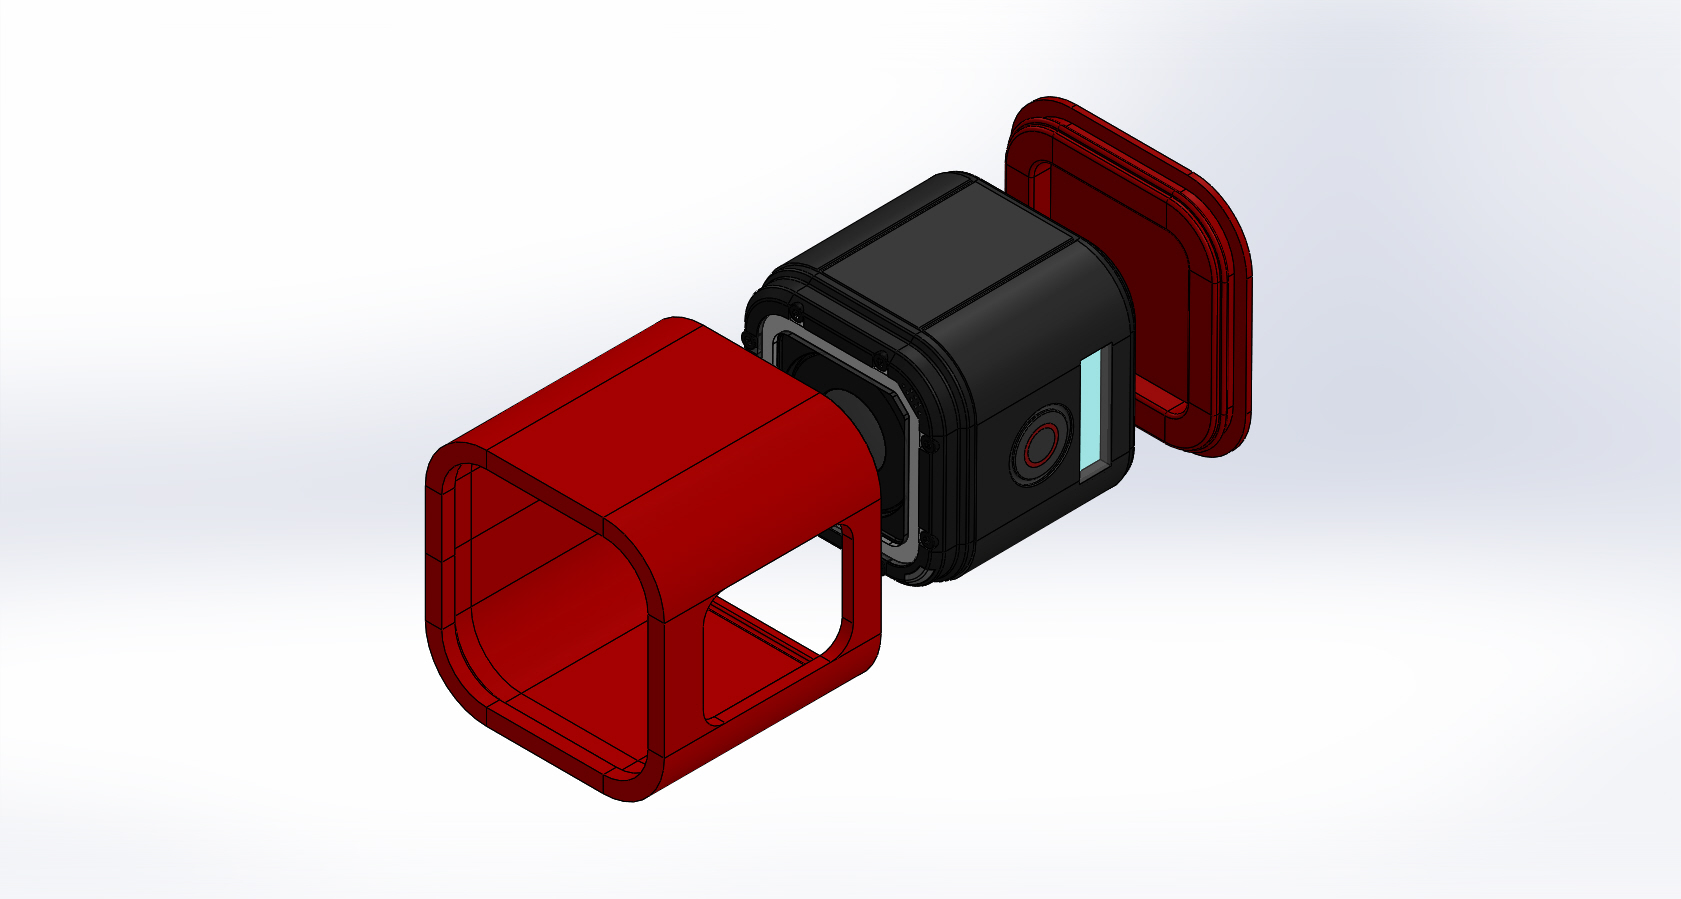
\includegraphics[width=\linewidth]{figures/sylvanexploded.JPG}
  \caption{Solidworks model of the GoPros Hero 4 Session}
  \label{fig:sylvancase}
\end{figure}

sdfgsdfgsdfg

\begin{figure}[!ht]
  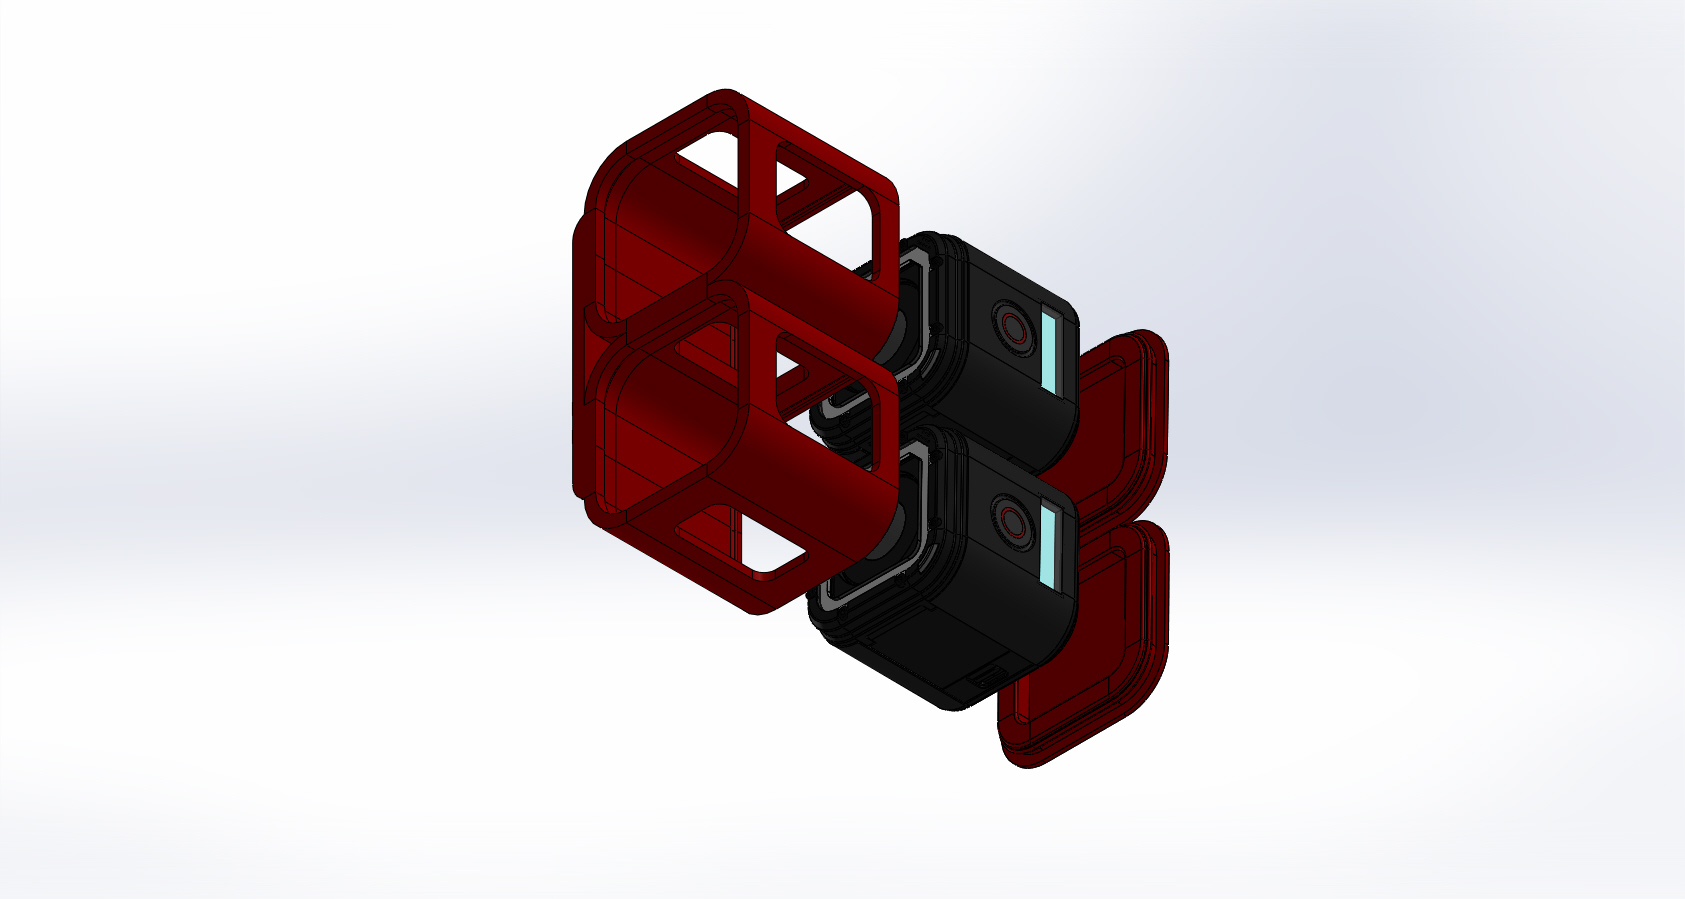
\includegraphics[width=\linewidth]{figures/stereoHolder1.JPG}
  \caption{angle 1}
  \label{fig:finalcase1}
\end{figure}

adsfasdfsdfg


\begin{figure}[!ht]
  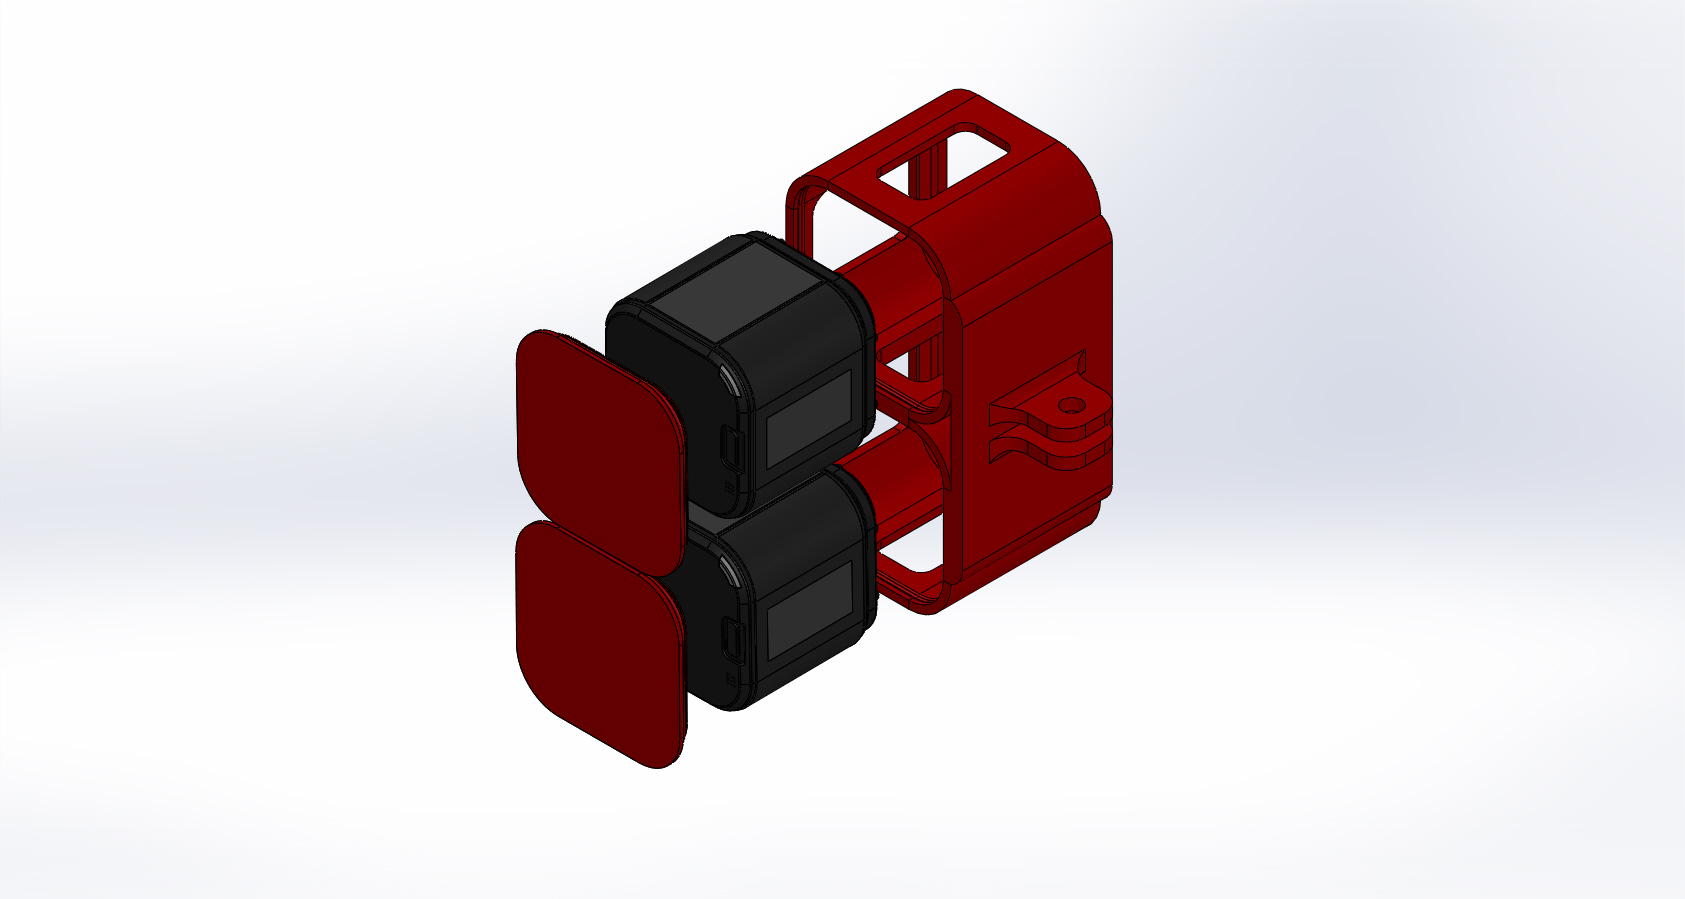
\includegraphics[width=\linewidth]{figures/stereoHolder2.JPG}
  \caption{angle 2}
  \label{fig:finalcase2}
\end{figure}

sdfgsdfgdsf

\begin{figure}[!ht]
  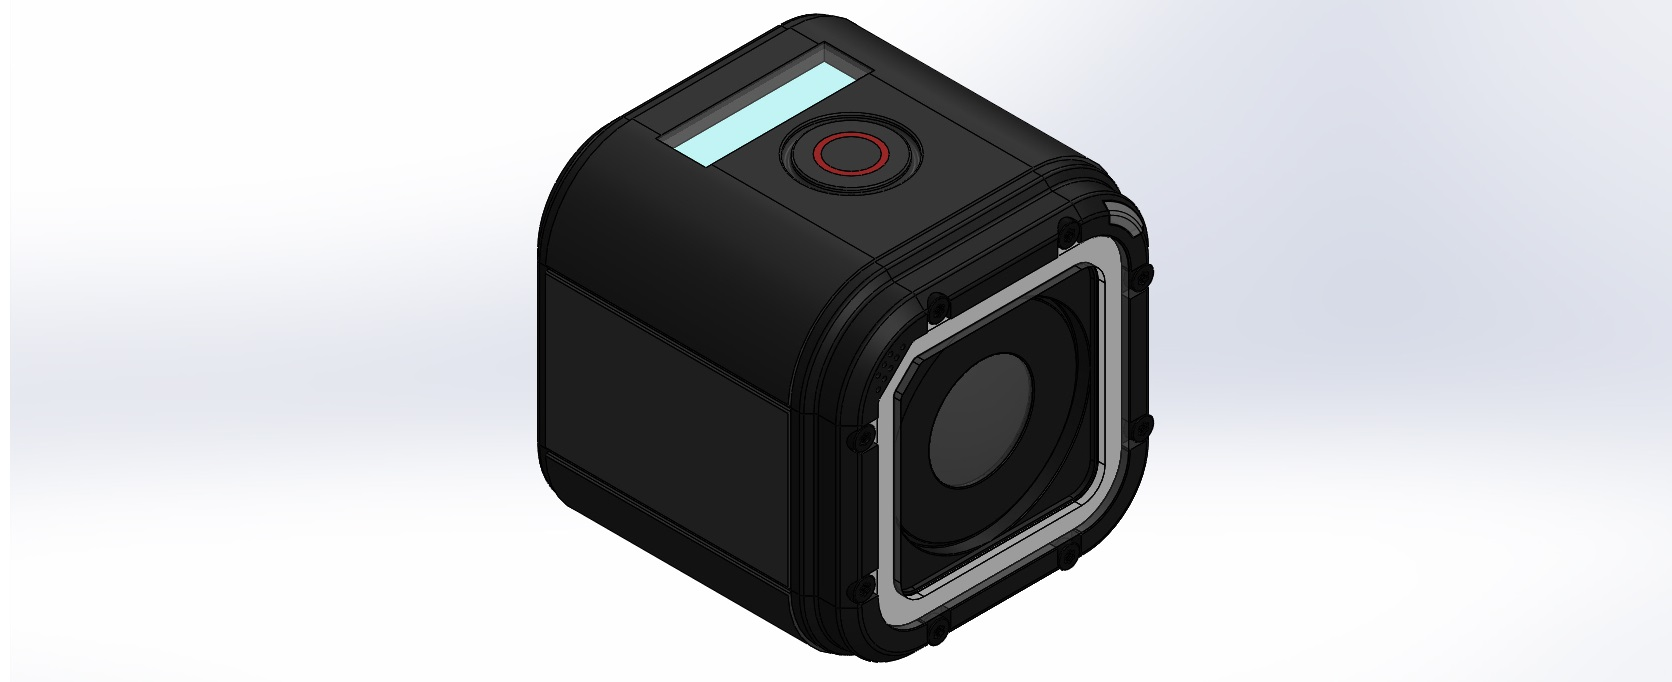
\includegraphics[width=\linewidth]{figures/GoProHero4Session.JPG}
  \caption{Solidworks model of the GPHS Action Camera from \cite{gph4smodelgrabcad}}
  \label{fig:goproherosession4}
\end{figure}

sdfgdsfgdsfg








\section{Vision Calibration}


matlab stereo camera calibration software
1. calibrate the cameras
2. get data from the recordings

took some vids

made matlab script to isolate frames in vids

put frames into stereo video camera calibrator

winning at life


